\documentclass[12pt]{article}
\usepackage[margin = 1in]{geometry}
\usepackage[USenglish]{babel}
\usepackage{natbib}
\usepackage{amsmath}
\usepackage{graphicx}
\usepackage{setspace}
\usepackage{subcaption}
\usepackage{xcolor}
\usepackage{titletoc}
\usepackage[colorlinks=true,citecolor=red!50!black,urlcolor=blue!50!black,linkcolor=red!50!black]{hyperref}

% sans serif font
\renewcommand{\familydefault}{\sfdefault}

\title{Measuring Morality in Political Attitude Expression}
\author{\textbf{Patrick W. Kraft}\\Ph.D. Candidate\\Department of Political Science\\Stony Brook University\\ Stony Brook, NY 11794\\\href{mailto:patrick.kraft@stonybrook.edu}{patrick.kraft@stonybrook.edu}}
\date{}


\begin{document}
\maketitle
\doublespacing
\thispagestyle{empty}

\begin{center}\large
Conditionally accepted at the \textit{Journal of Politics}\\
\textit{Short title:} Measuring Morality
\end{center}

\clearpage\thispagestyle{empty}
\begin{abstract}
This study explores whether and how individuals evoke moral considerations when discussing their political beliefs. Analyzing open-ended responses in the 2012 American National Election Study (ANES) using a previously validated dictionary, I find systematic ideological differences in moral reasoning---even when respondents are not explicitly asked about morality. The study proceeds to show that the reliance on moral considerations in attitude expression is amplified by the moral content of individual media environments.

\vspace{\baselineskip}
\noindent \textbf{Keywords:} Moral Foundations Theory, Open-ended Survey Responses, Text Analysis, Media Contents

\vspace{\baselineskip}
\noindent \textbf{Online Appendix:} Supplementary material for this article is available in the appendix in the online edition.

\vspace{\baselineskip}
\noindent \textbf{Replication files:} Replication files are available in the JOP Data Archive on Dataverse (\url{http://thedata.harvard.edu/dvn/dv/jop}) as well as on GitHub (\url{https://github.com/pwkraft/mft}).
\end{abstract}


\newpage
\setcounter{page}{1}

Increasing levels of polarization have renewed scholarly interest in the psychological and attitudinal differences between liberals and conservatives \citep{jost2006end}. One such area of research focuses on the moral underpinnings of ideology. According to \textit{Moral Foundations Theory} (MFT), moral thinking is organized by at least five dimensions: care/harm, fairness/cheating, loyalty/betrayal, authority/subversion, and sanctity/degradation \citep{graham2013moral}. Liberals and conservatives differ in their emphasis on each foundation, with liberals prioritizing care and fairness, and conservatives endorsing all five dimensions equally \citep{graham2009liberals}.

A series of recent studies shows that the moral foundations influence issue preferences \citep{kertzer2014moral}, candidate trait evaluations \citep{clifford2014linking}, and vote choice \citep{iyer2010beyond}. Research further suggests that moral framing in elite communication can elicit attitude change \citep[e.g.][]{clifford2015concerns,feinberg2013moral}. For the most part these studies measure moral reasoning with the Moral Foundations Questionnaire (MFQ), which explicitly asks respondents to judge the importance of considerations related to the five foundations \citep[e.g.,][]{graham2011mapping}. Yet, by explicitly asking about morality, researchers presuppose an important link that requires more careful empirical investigation.

The present study explores how people utilize moral arguments in day-to-day political reasoning in a more unobtrusive context. Using a moral dictionary validated in previous studies \citep{graham2009liberals}, I propose a novel approach to analyze individual verbatim responses to open-ended likes/dislikes questions in the 2012 American National Election Study (ANES). Measuring moral reasoning in open-ended responses directly captures whether political attitudes are infused by morality without being prompted by the language of a questionnaire. Insofar as moral intuitions play a role in political attitude expression, citizens should rely on the moral foundations when discussing their opinions about political actors, even if not explicitly asked to do so.

The analysis begins by replicating previous findings regarding MFT and ideology using the open-ended measure. Consistent with MFT, the results reveal systematic differences between liberals and conservatives in the reliance on specific moral considerations. Furthermore, these differences in verbatim moral reasoning predict candidate preferences and vote choice---even after controlling for a person's party identification. Integrating a large-scale content analysis of individual media environments, I proceed to show that people who are exposed to moral rhetoric in political news are more likely to rely on moral considerations when discussing their political beliefs. Overall, this study improves conventional dictionary-based approaches to analyze open-ended responses and showcases the integration of individual media environments to trace the influence of media exposure on attitude expression.


\section*{Method}

This study utilizes the moral foundations dictionary created by \citet{graham2009liberals} to identify references to specific moral considerations when respondents discuss what they like and dislike about political parties and candidates.\footnote{See Appendix A for the full content of the dictionary.} Other studies have used (variations of) this dictionary to identify the moral foundations in elite communication \citep[e.g.,][]{clifford2015concerns} or political advertising \citep[e.g.,][]{lipsitz2017playing}, but to date no research has examined verbatim attitude expressions in surveys. Based on the terms signaling each foundation in the dictionary, any document can be scored according to its emphasis on the respective moral dimension. Conventional dictionary-based methods usually consist of the proportion of signal word occurrences in each document \citep[e.g.,][]{graham2009liberals}. However, some dictionary terms are problematic when applied to verbatim survey responses. In particular, certain words might be too ubiquitous to be regarded as an unambiguous indicator for specific moral considerations. For example, ``leader'' is a signal word for the authority dimension. However, respondents may describe the qualities of presidential candidates as \textit{leaders} irrespective of moral considerations related to authority.

One way to address this problem would be to revise the dictionary and eliminate ambiguous words. Yet such revisions could be arbitrary and leave too much discretion to the researcher. Drawing on techniques developed in the field of information retrieval, I propose an alternative approach. If a specific dictionary term like ``leader'' is commonly used to describe presidential candidates, it is likely that the term can be used in multiple contexts and is not necessarily unique to the moral domain. Terms that are used by almost all respondents therefore provide less information about differences in their (moral) reasoning than terms that only occur in few responses. In this study, \textit{MFT scores} are computed for a foundation by weighting each term in the dictionary according to its ubiquity across documents, which serves as a proxy for the term's discriminative information:
\begin{equation}\label{eq:tfidf}
\text{MFT}_{if} = \dfrac{1}{W_i} \sum_{t \in \mathcal{D}_f} \left[ w_{it} * \log_{10}\left( \dfrac{N}{n_t}\right) \right],
\end{equation}
where $\text{MFT}_{if}$ denotes the score of document $i$ for foundation $f$, $W_i$ is the total number of words in document $i$, $t$ indicates a term in the set of signal terms in foundation dictionary $\mathcal{D}_f$, $w_{it}$ denotes the number of occurrences of term $t$ in document $i$, $N$ represents the total number of documents, and $n_t$ is the number of documents in which the term $t$ appears. The weight represents the inverse of the proportion of documents in which the target term appears.\footnote{This specification is usually referred to as tf-idf weighting and is commonly used in quantitative text analysis (see \citealt[ch. 6]{manning2008introduction} for an introduction).} Terms that are ubiquitous across the entire corpus receive a lower weight, and terms that appear in only few documents receive a higher weight. %The denominator includes $+1$ to ensure that it does not equal zero if a dictionary term does not appear in any document.

Each document is an individual's verbatim response to a set of open-ended questions. As such, a respondent's MFT score for foundation $f$ is the weighted proportion of words in the response that signal the respective foundation. The score has a lower bound of 0 (document does not contain any dictionary terms) and is independent of document length (since it is based on relative occurrences). Higher scores imply larger proportions of dictionary terms in a document. Most importantly, however, words that appear in nearly all open-ended remarks affect MFT scores less than words that appear only in a few responses because ubiquitous terms convey less information about differences across individuals. Overall, the MFT score provides a correction for potential distortions due to suboptimal terms in the dictionary. Since nominal values of the MFT score above zero do not have a clear substantive interpretation, they are rescaled to unit variance.


\section*{Results}

Open-ended responses to the likes/dislikes items in the 2012 ANES were aggregated for each individual and pre-processed by correcting spelling errors before computing MFT scores. Appendix B provides detailed information on the procedure, including the weighting scheme and raw proportions of individuals mentioning each foundation. Results for the sanctity dimension are not presented below due to its low general prevalence in individual attitude expressions.\footnote{Only about 3.6\% of respondents mentioned the sanctity dimension.} To account for confounding factors related to the respondents' eloquence when discussing their political attitudes, all models reported below include controls for education, logged overall response length, as well as the Wordsum vocabulary score measuring verbal intelligence.


\subsection*{Ideological Differences}

MFT scores measure the weighted proportion of moral foundation terms in an open-ended response. Since they are bounded at zero (i.e., response does not contain any moral words), I begin by estimating a set of Tobit regressions using ideology to predict individual MFT scores for each moral foundation.\footnote{Full estimates for this and all subsequent models are presented in Appendix D.} Figure~\ref{fig:tobit_ideol} compares liberals and conservatives while holding all other variables constant at their respective means. To facilitate their substantive interpretation, I decompose the estimates into the effect of ideology on the probability of mentioning a specific foundation \textit{at all} (i.e., the probability the MFT score is larger than zero) as well as the degree of emphasis on the foundation given that it was mentioned by a respondent (i.e., the change in the MFT score given that it is larger than zero, measured in standard deviations).\footnote{See for example \citet{mcdonald1980uses} for details on decomposing Tobit estimates.}

\begin{figure}[ht]\centering
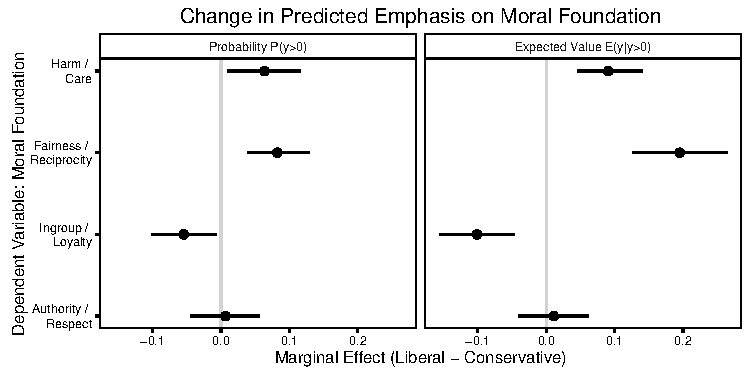
\includegraphics{../calc/fig/tobit_ideol.pdf}
\caption{Difference between liberals and conservatives in the probability of mentioning a moral foundation (left panel) and in the MFT score given that the foundation was mentioned (right panel), holding control variables at their respective means (along with 95\% confidence intervals). Control variables include age, sex, race, church attendance, survey mode, education, response length, and the Wordsum vocabulary score. Full model results are displayed in Appendix D.1.
}\label{fig:tobit_ideol}
\end{figure}

Positive values denote a higher probability of mentioning the respective moral foundation (left panel) or a higher MFT score (right panel) among individuals who identified as liberals, while negative values indicate a higher probability/higher score among conservatives. The effects are consistent with the expectations of MFT for three out of four moral foundations. Liberals are about 8 percentage points more likely than conservatives to mention the foundations of care and fairness. Furthermore, given that respondents mention these two foundations at all, liberals emphasize it more than conservatives when evaluating political parties and candidates. The MFT score for the care foundation is about 0.12 standard deviations higher among liberals than conservatives. The effect is slightly larger for the fairness dimension. Conversely, being conservative is associated with an increased loyalty MFT score by about 0.1 standard deviations. There are no significant differences between liberals and conservative on the authority dimension.


\subsection*{Moral Considerations and Vote Choice}

A skeptic may worry that the verbal expression of moral considerations might not be as strongly related to other forms of political behavior (e.g., vote choice) as moral foundations measured by the MFQ. To address this concern, Figure~\ref{fig:logit_vote} presents the changes in expected probabilities of voting for the Democratic (vs. Republican) presidential candidate in the 2012 election for individuals emphasizing the moral foundations in their open-ended responses. The estimated probabilities are based on logit models including MFT scores for each moral foundation as independent variables as well as controls for various sociodemographic characteristics. Individuals who emphasized moral considerations related to the care and fairness foundations were more likely to vote for Barack Obama than for Mitt Romney. Respondents who emphasized the loyalty foundation, on the other hand, were less likely to vote for Obama.\footnote{Appendix C.3 shows similar results in an analysis of feeling thermometers towards parties and candidates.}

\begin{figure}[ht]\centering
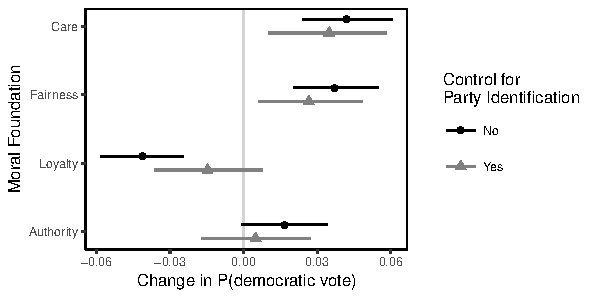
\includegraphics[scale=.9]{../calc/fig/logit_vote.pdf}
\caption{Change in predicted probabilities of voting for the Democratic rather than Republican candidate when MFT score is increased from its minimum (no overlap between dictionary and response) by one standard deviation, holding control variables constant at their respective means (along with 95\% confidence intervals). Control variables include party identification, age, sex, race, church attendance, survey mode, education, response length, and the Wordsum vocabulary score. Full model results are displayed in Appendix D.2.
}\label{fig:logit_vote}
\end{figure}

The effects on vote choice might not seem large, but bear in mind that the measure of moral reasoning is based solely on the content of open-ended responses in which respondents were \textit{not} explicitly asked about morality. The fact that moral considerations evoked by respondents are nevertheless related to their political preferences indicates that their open-ended comments about both candidates and parties are imbued with moral content that in turn relates to political judgments in the manner suggested by MFT. As such, analyzing \textit{how} individuals talk about their political preferences prior to an election helps us predict their subsequent vote choice.


\subsection*{Media Content and Exposure to Moral Rhetoric}

It can also be informative to examine the reliance on moral considerations \textit{in general} rather than focusing only on individual foundations. For example, a recent study found that moral language in political ads elicits emotional responses among recipients \citep{lipsitz2017playing}. Here, I investigate whether exposure to moralized discourse in the media is associated with a stronger general reliance on moral considerations in attitude expression. For each individual, I compute the sum of MFT scores to measure emphasis of \textit{any} moral foundation. The main independent variable captures moralization of media environments based on a content analysis of media sources consumed by each individual. Using Lexis-Nexis, I retrieved the content of 28 media sources covering either presidential candidate during the survey field period in the last month of the campaign (October 2012) and coded the emphasis on moral considerations using the weighted dictionary approach described earlier.\footnote{Sources include e.g., New York Times, CNN.com, and Fox News Programs. See Appendix B for details.} Based on each source's content, I create a measure that represents the extent to which each individual's media environment emphasized moral considerations by averaging (median-centered) MFT scores of all media outlets retrieved by a respondent.

\begin{figure}[h]\centering
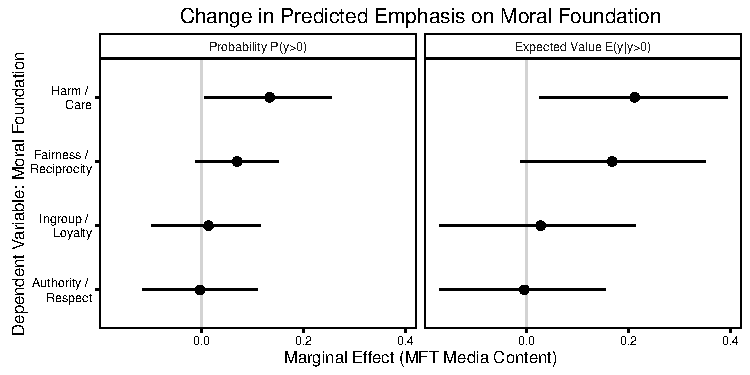
\includegraphics{../calc/fig/tobit_media.pdf}
\caption{Effect of MFT content in individual media environments on the probability of mentioning any moral foundation (left panel), and on the summed MFT score given that any foundation was mentioned (right panel), holding control variables at their respective means (along with 95\% confidence intervals). Control variables include political knowledge, general media exposure, political discussion frequency, age, sex, race, church attendance, survey mode, education, response length, and the Wordsum vocabulary score. Full model results are displayed in Appendix D.3.
}\label{fig:tobit_media}
\end{figure}

Figure~\ref{fig:tobit_media} presents the results of a Tobit model where effects are again decomposed into the probability of mentioning any moral foundation (left panel) as well as the emphasis on morality, given that any foundation was mentioned (right panel). Individuals who are exposed to media sources that report on the campaign in a more moralized manner put a stronger emphasis on moral considerations in their open-ended responses. Although it is difficult to determine the causal ordering, the pattern is consistent with research suggesting that people adopt moral arguments from their media environment \citep[e.g.,][]{clifford2015concerns}. 


\subsection*{Robustness Checks}

To this point, the analyses assume that the dictionary-based approach captures the theoretical concept of interest---\textit{morality}. Yet, the terms in the dictionary may also be recovering other (i.e., non-moral) patterns in word choice. Appendix C presents the results of multiple supplementary analyses to alleviate this concern for both open-ended responses as well as media environments. Two results are briefly highlighted here.

First, could the ideological differences in open-ended responses be explained by the survey context? To test for this possibility, I replicate the analysis from Figure~\ref{fig:tobit_ideol} using data from a random-digit-dial adult sample of residents within a 25 mile radius of a large northeastern state university conducted between early January, 2001 and July, 2003. Compared to the ANES, the survey varied the mode (phone), political context (non-election year, Republican presidency), as well as the set of open-ended items (discussing liberals and conservatives as social groups rather than candidates and parties). Notwithstanding these changes, the ideological differences in moral reasoning are consistent with the results presented above.

Second, even if the patterns can be replicated, can the dictionary really capture underlying moral rhetoric? In an additional analysis, I compare dictionary-based MFT scores with individual assessments of moralization conducted by an independent group of researchers. \citet{feinberg2013moral} explored moral rhetoric in a set of 232 newspaper op-eds on environmental issues by asking a group of coders to assess the degree to which they used rhetoric grounded in moral foundations. Moralization measured using MFT scores is positively correlated with individual coder assessments that did not rely on any dictionary (although modestly, $r=0.27$).


\section*{Discussion}

Moral Foundations Theory has become an influential framework for understanding ideology and political attitudes. Yet, existing measures fail to directly assess whether individuals rely on moral considerations in their day-to-day political reasoning. I address this gap by examining moral arguments in individual attitude expression. Consistent with MFT, there are systematic patterns in the emphasis on moral considerations among liberals and conservatives for three out of four foundations. Liberals are more likely to mention considerations related to care and fairness, whereas conservatives are more likely to emphasize the moral foundation of loyalty. Moreover, morality in attitude expression is related to vote choice and the exposure to moralized political discourse in the mass media is associated with increased reliance on moral considerations.

That said, ideological differences on binding foundations (loyalty, authority) appear less persistent than those on individualizing foundations (care, fairness). Appendix C.2 examines potential explanations by analyzing subsets of the dictionary and the open-ended items. Liberals are more likely to mention the authority foundation in the context of positive moral endorsements (\textit{virtues}) when they discuss aspects they \textit{liked} about their \textit{in-party}. In contrast, there is suggestive evidence that conservatives are more likely to discuss the authority dimension in the context of negative endorsements (\textit{vices}). This finding indicates that liberals and conservatives attach diverging meanings to certain foundations, which promises to be a fruitful area for future research.

Overall, this study improved conventional dictionary-based approaches in order to utilize a largely neglected data source: verbatim open-ended responses. Using this method, scholars can study moral reasoning in surveys that do not contain the MFQ simply by relying on open-ended items. Lastly, the approach outlined here allows for a seamless integration of media content in the analysis of moral reasoning, which can further illuminate how exposure to political discourse fosters ideological differences in moral reasoning. In times of growing partisan polarization, a better understanding of the antecedents of this ideological divide is essential.

\bibliographystyle{apsr2006short}
\bibliography{mft_lit}

\section*{Acknowledgments}
I thank Jennifer Jerit, Yanna Krupnikov, Stanley Feldman, Jason Barabas, Hannah Nam, Reuben Kline, Peter DeScioli, Fridolin Linder, Scott Clifford, 
Robert Klemmensen, three anonymous reviewers, and participants at the panel of the 2015 Annual Meeting of the Midwest Political Science Association for helpful comments on earlier versions of this paper. Special thanks to Leonie Huddie as well as Matthew Feinberg and Robb Willer for sharing their data.

\section*{Biographical Statement}

Patrick W. Kraft is a Ph.D. candidate in the Department of Political Science at Stony Brook University, Stony Brook, NY 11794.

\end{document}